\section{Diagrams}

The diagram on Figure 3 shows what happens when a user is interested by a service. First the user click on the 'Accept' button of this service (aService in the Figure 3), then we add this user in the list of users interested in this service.
\\ If this user is the first on this list, the server do a transaction, update the service then we add this transaction to the "transactions historic" of both the user and the creator of this service.
\\ Finally, we send a message from the customer to the creator to let him know his interest. We do this in every case because we want to let the creator know about all the followers. It can be interesting, for example, if the first customer of the list didn't manifest after a long time, the creator know the other customer and then can contact them.

\begin{figure}[!ht]
	\begin{center}
		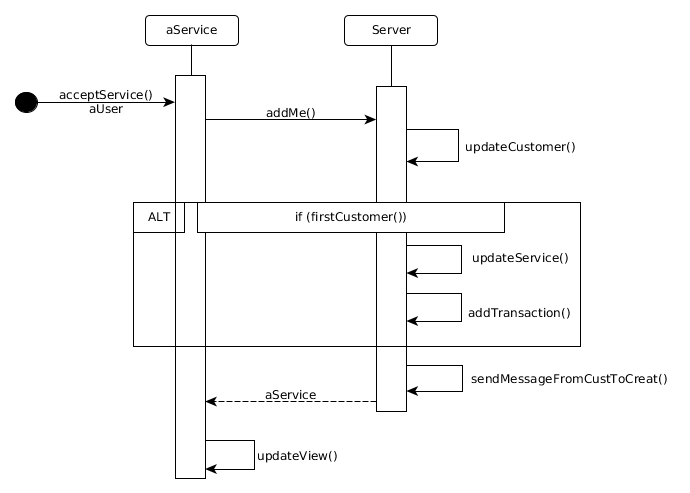
\includegraphics[width=\textwidth]{seq_acceptService.png}
		\caption{Sequence Diagram : Acceptance of an offer or a demand}
		\label{fig:acceptService}
	\end{center}
\end{figure}

The diagram on Figure 4 shows what happens when a user creates a service (an offer or a demand). After fulfilling the form and checking the integrity of the form. We send to the server the date, the server will then send an object service (aService in the Figure 4). We then give to the creator the opportunity of sharing this service with an eventual group and/or on a social network. 
\\ Meanwhile, we will do an automatic search to see if there is already an offer/demand in the database that can match this new service and show the results to the creator.

\begin{figure}[!ht]
	\begin{center}
		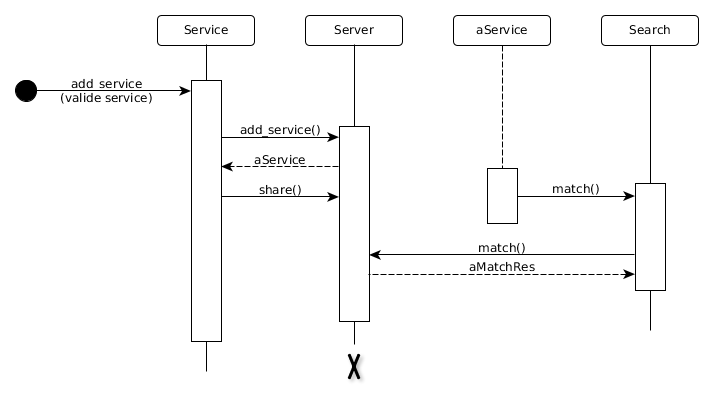
\includegraphics[width=\textwidth]{seq_addService.png}
		\caption{Sequence Diagram : Creation of an offer or a demand}
		\label{fig:addService}
	\end{center}
\end{figure}

\newpage
In the Figure 5, we show the creation of a user account on the website. An unregistered user, after fulfilling the form and after we check its integrity, push the "create Account" button. We send the data from the form to the server, the server then add this new user to the DataBase. 
\\ Then, it sends back a 'user object', an object that contains all the information that the user gives us plus his ID. With this information, we can show the Profile of the user.

\begin{figure}[!ht]
	\begin{center}
		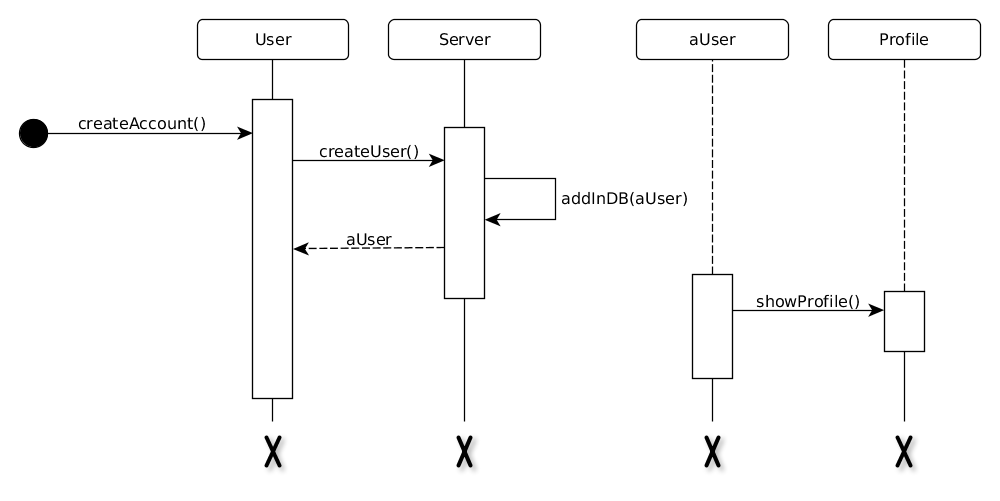
\includegraphics[width=\textwidth]{seq_createUser.png}
		\caption{Sequence Diagram : Creation of an account on the website}
		\label{fig:createUser}
	\end{center}
\end{figure}

In the Figure 6, we show the possibilities give to the user when he perform a search. After taking the data from the search form, the server performs a match and send back the results.
Once we have the results, we can do several things.
\begin{itemize}
	\item SORTED : With this action, the user can order the results by differents fields (date, creator, title, tag, ...)  in a decreasing or increasing order. We order in a dynamic way in this way we have less request on the server.
    \item FOLLOW : With this action, the user can add himself in the list of the followers of this service. A follower is always informed of the modifications on the service.
    \item QUICKS : With this action, the user can accept a service.  In our server, we perform this action by adding a new service that match with the request of the user.  After that, we perform the sames actions that we explain in Figure 1 : accept a service.
    
\end{itemize}

\begin{figure}[!ht]
	\begin{center}
		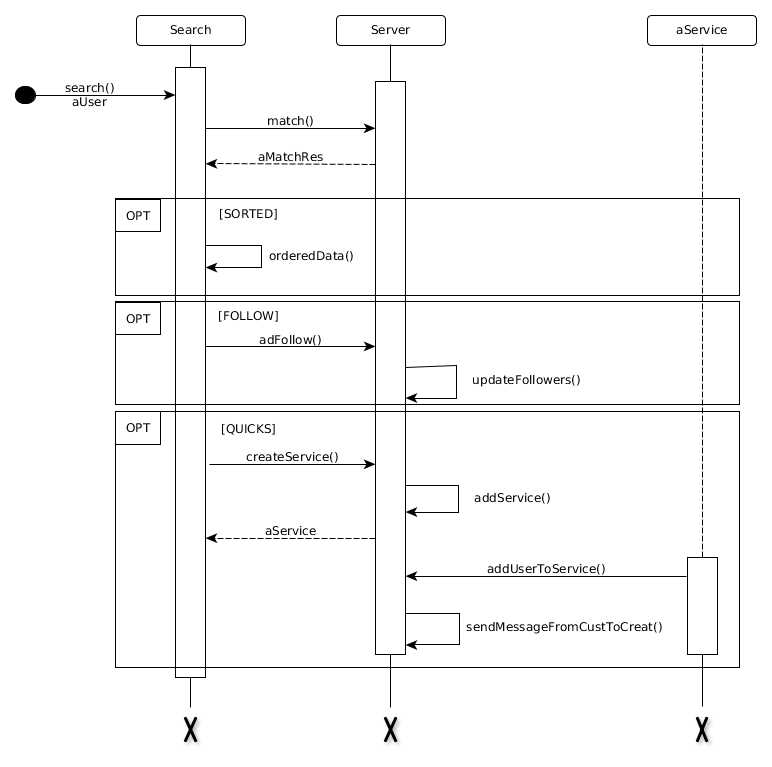
\includegraphics[width=\textwidth]{seq_search.png}
		\caption{Sequence Diagram : The procedure of a search}
		\label{fig:search}
	\end{center}
\end{figure}

On the Figure 7, we show what happens when a service is finished, ie when the customer and the creator met and performed the service.
\\ When it's finished, the creator and/or the customer can send a cotation with a optional message. 
\\ We get this informations from a form, the server then update the service, add karma (ie the cotation) to the customer or the creator and add the message to the 'transactions history' of the customer or creator.
\\ If the customer and the creator have given a cotation, we ask to server the list of all other user interested by the service and send them a message to warn them that the offer/demande is not available anymore. After that, we archive the service.
\\ If the customer or the creator didn't give a cotation, we send them a message and ask them to give one as soon as possible.

\begin{figure}[!ht]
	\begin{center}
		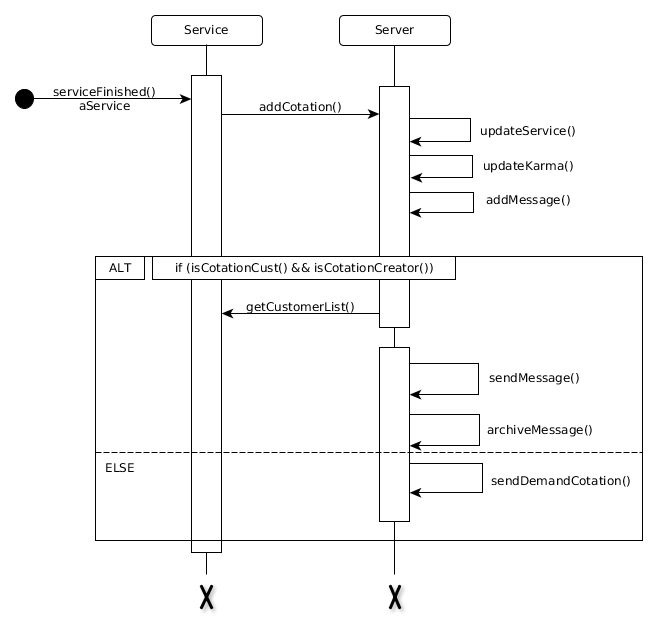
\includegraphics[width=\textwidth]{seq_serviceFinished.png}
		\caption{Sequence Diagram : End of a Service, Cotation and Karma}
		\label{fig:serviceFinished}
	\end{center}
\end{figure}


\begin{landscape}

\begin{figure}[!ht]
	\begin{center}
		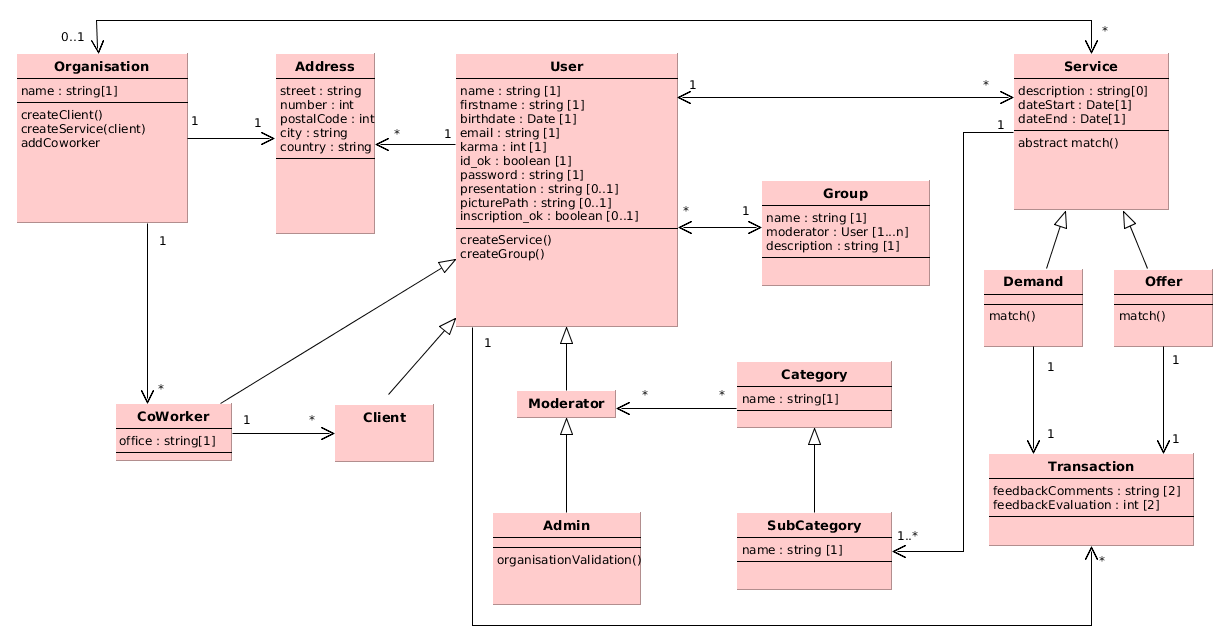
\includegraphics[width=.85\paperheight]{UML.png}
		\caption{Unified Modeling Language (UML): class diagram}
		\label{fig:uml}
	\end{center}
\end{figure}


\end{landscape}